\section{Introduktion}
{%
	\begin{frame}{Problem} % the plain option removes the sidebar and header from the title page
\begin{itemize}
	\item PsyLog som platform
	\item Jørgen Aagaard: Søvn og social aktivitet er vigtige faktorer
	\item Vi beskæftiger os med social aktivitet
	\begin{itemize}
		\item Depression - mindsket social aktivitet
		\item Mani - forhøjet social aktivitet
		\item Muligt at observere patient via social aktivitet på mobilen
	\end{itemize}
	\item Ingen tilgængelig forskning der foreslår en model
\end{itemize}

\end{frame}}


{ %
	\begin{frame}{Mål for projekt} % the plain option removes the sidebar and header from the title page
		Vi vil gøre det muligt at udføre psykiatrisk forskning på området
		\begin{itemize}
			\item Social aktivitet
			\begin{itemize}
				\item Social aktivitet på telefonen
				\item Log så meget data som muligt
			\end{itemize}	
			\item Stemningsleje
			\begin{itemize}
				\item Metoder der svarer til nuværende lægepraksis
			\end{itemize}
		\end{itemize}
	\end{frame}}
	



{ %
	\begin{frame}{Eksisterende forskning} % the plain option removes the sidebar and header from the title page
		Få kilder i psykiatrisk forskning benytter mobile sensorer
		Social Sensing for Epidemiological Behaviour Change
		\begin{itemize}
			\item 70 Studerende på et kollegium
			\item Opkadshistorik, SMS-historik, WLAN lokation samt Bluetooth interaktioner
			\item Resultater:
			\begin{itemize}
				\item Sammenhæng mellem antal sociale interaktioner og fysisk/psykisk sygdom
				\item Individer med færre interaktioner meldte ``sad / lonely / depressed''
			\end{itemize}
		\end{itemize}
		
		
	\end{frame}}

\section{Ikke-forstyrrende dataopsamling}
{ %
	\begin{frame}{Ikke-forstyrrende dataopsamling} % the plain option removes the sidebar and header from the title page
		Muligheder for ikke-forstyrrende dataopsamling
		\begin{itemize}
			\item \textbf{Opkald}
			\item \textbf{SMS}
			\item Lokation
			\item E-mail
		\end{itemize}
			
	\end{frame}}



{ %
\begin{frame}{Analyser} % the plain option removes the sidebar and header from the title page
Følgende analyser vurderes brugbare for opkald og sms/mms
\begin{itemize}
	\item \textbf{Antal samtaler} - flere samtaler tyder på mere interaktion
	\item \textbf{Samtalelængde / beskedlængde} - lange samtaler tyder på dybere interaktion
	\item \textbf{Antal forskellige kontakter} - flere kontakter tyder på lyst til at have kontakt med andre
	\item \textbf{Mistede opkald / intet svar} - mistede opkald tyder på indelukket patient
\end{itemize}
	
\end{frame}}

\section{Forstyrrende dataopsamling}

{ %
\begin{frame}{PANAS} % the plain option removes the sidebar and header from the title page
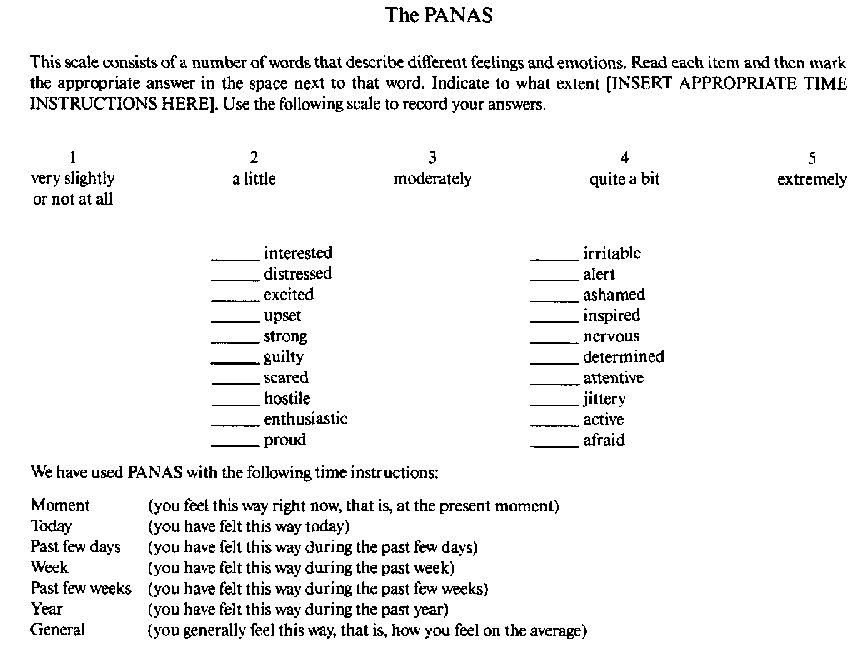
\includegraphics[width=\textwidth]{panas}
	
\end{frame}}

{ %
	\begin{frame}{Stemningsregistrering} % the plain option removes the sidebar and header from the title page
		Patienten reflekterer over sit eget stemningsleje
		
		\begin{center}
		\begin{tabular}{|c|}
			\hline \cellcolor{red!90} Svær mani \\ 
			\hline \cellcolor{red!60} Moderat mani \\ 
			\hline \cellcolor{red!30} Let mani \\ 
			\hline \cellcolor{yellow!70} Normal \\ 
			\hline \cellcolor{blue!30} Let mani \\ 
			\hline \cellcolor{blue!60} Moderat mani \\ 
			\hline \cellcolor{blue!90} Svær mani \\ 
			\hline 
		\end{tabular} 
		\end{center}
	\end{frame}}
	
{ %
	\begin{frame}{Stemningsregistrering} % the plain option removes the sidebar and header from the title page

		Angst specificeres på følgende skala:
		\begin{tabular}{| c | l|}
			\hline 0 & Ingen angst \\ 
			\hline 1 & lettere angst der ikke påvirker hverdagen\\ 
			\hline 2 & Konstant angst, funktionsniveau påvirkes\\ 
			\hline 3 & Udtalt angst, kan næsten ikke foretage sig noget\\
			\hline
		\end{tabular} 
	\end{frame}}
	
{ %
	\begin{frame}{Stemningsregistrering} % the plain option removes the sidebar and header from the title page
		
		Derudover noteres detaljer om patientens hverdag
		\begin{itemize}
			\item Antal timers søvn
			\item Medicinforbrug
			\item Vægt
			\item Menstruation
		\end{itemize}
	\end{frame}}
	
{ %
\begin{frame}{Hamilton Depressionsskala} % the plain option removes the sidebar and header from the title page
	\begin{itemize}
		\item En mængde faktorer besvares givet mellem 3 og 5 svarmuligheder
		\item Score beregnes
		\item Stemningsleje vurderes
	\end{itemize}
	
	Begræsning:
	\begin{itemize}
		\item Kræver uddannet psykiater at udføre
	\end{itemize}
	
\end{frame}}
	
{ %
	\begin{frame}{Eksempler på spørgsmål} % the plain option removes the sidebar and header from the title page
		 Arbejde og interesser
		\begin{itemize}
			\item Ingen problemer
			\item Været mindre interesseret i de daglige aktiviteter eller følt sig lidt besværet
			\item Har følt sig noget insufficient i sine daglige aktiviteter
			\item Har haft svært ved at udføre selv de mere rutineprægede aktiviteter
			\item Har ikke været i stand til at udføre de rutineprægede aktiviteter uden hjælp
		\end{itemize}
		
	\end{frame}}

\subsection{Behov}
{ %
\begin{frame}{Behov} % the plain option removes the sidebar and header from the title page
For at kunne udføre de tre nævnte metoder skal vi kunne stille følgende typer af spørgsmål


\begin{itemize}
	\item Angivelse af værdi på Likert-skala
	\item Fri tekst
	\item Valg mellem tekstuelle predefinerede svarmuligheder
	\begin{itemize}
		\item Skal kunne tillægges farver
	\end{itemize}
\end{itemize}
\end{frame}}

\subsection{Demonstration}
\begin{frame}{Demonstration af implementeret modul} % the plain option removes the sidebar and header from the title page
\centering

\includegraphics[height=0.8\textheight]{demo_1_Tom}
\end{frame}

\begin{frame}{Demonstration af implementeret modul} % the plain option removes the sidebar and header from the title page
	\centering
	
\includegraphics[height=0.8\textheight]{demo_2_Noti}
\end{frame}

\begin{frame}{Demonstration af implementeret modul} % the plain option removes the sidebar and header from the title page
	\centering
	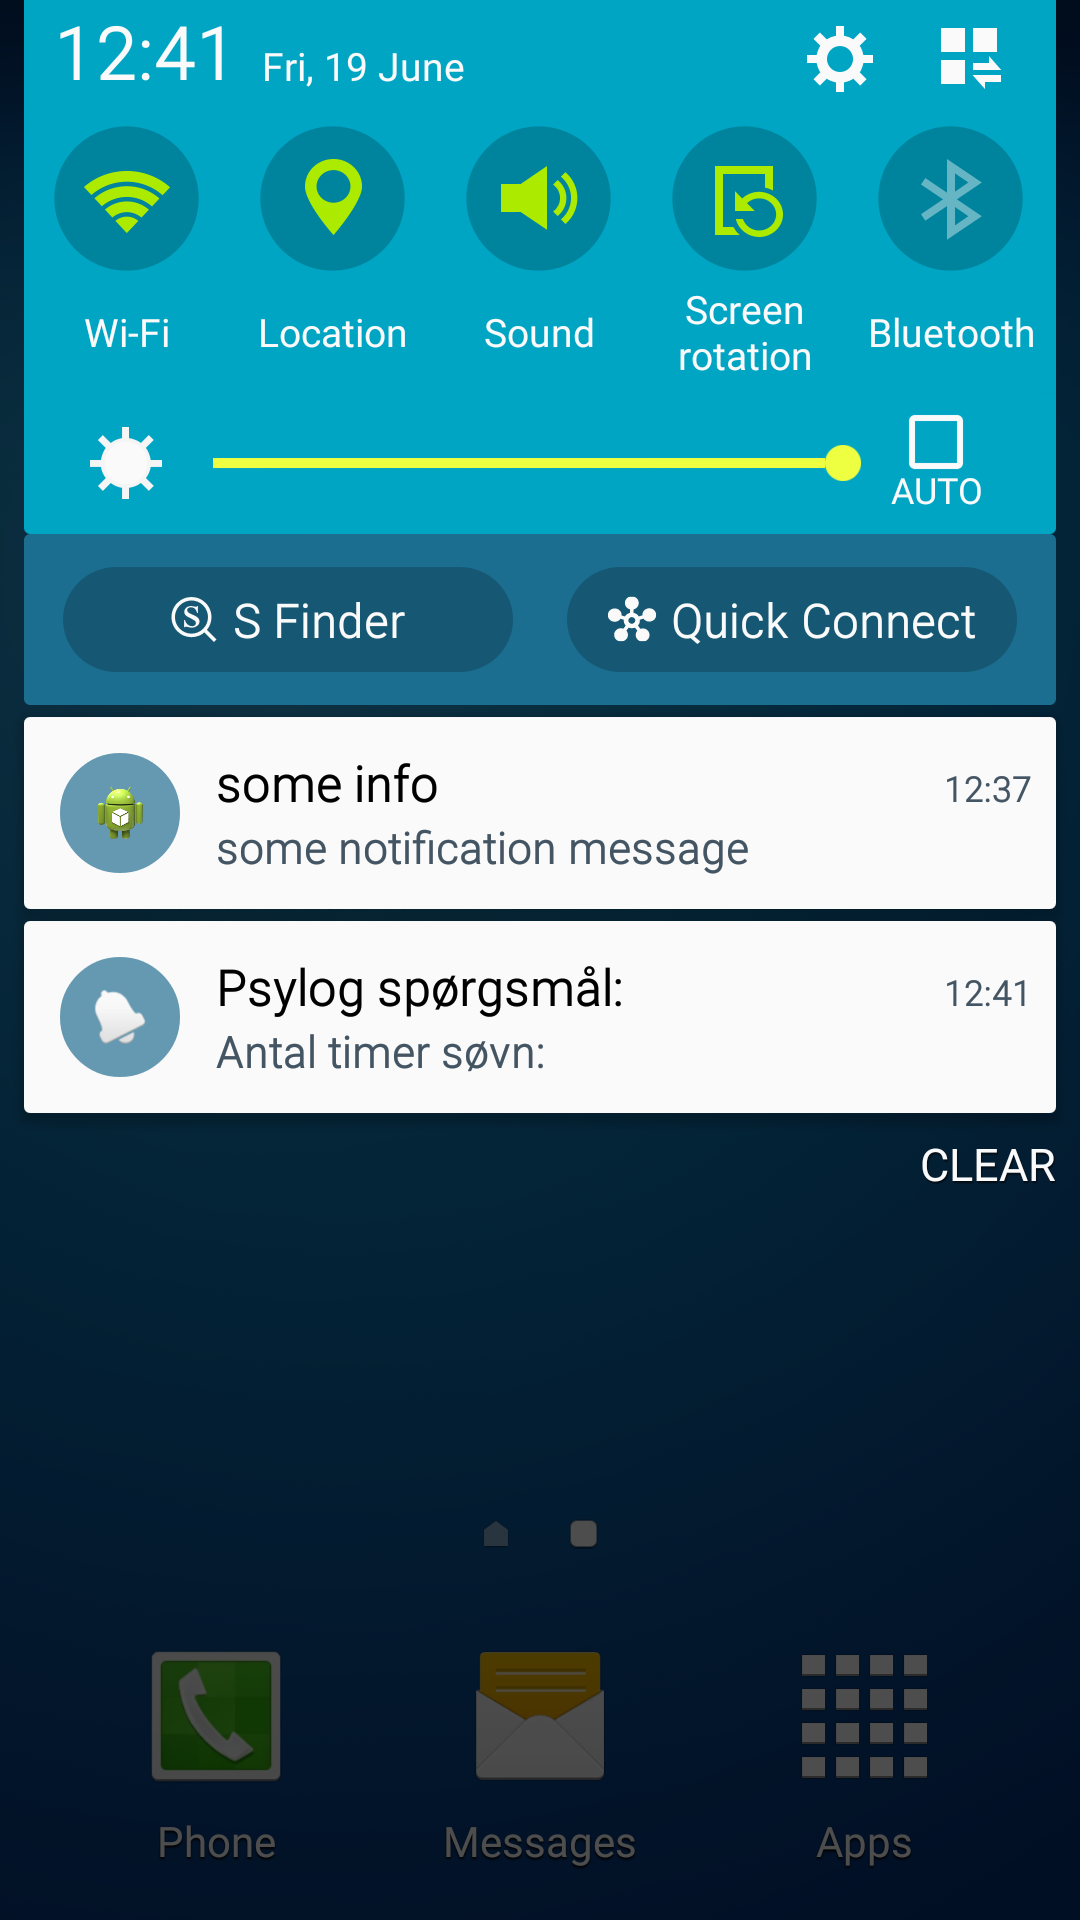
\includegraphics[height=0.8\textheight]{demo_3_Detaljer}
\end{frame}

\begin{frame}{Demonstration af implementeret modul} % the plain option removes the sidebar and header from the title page
	\centering
	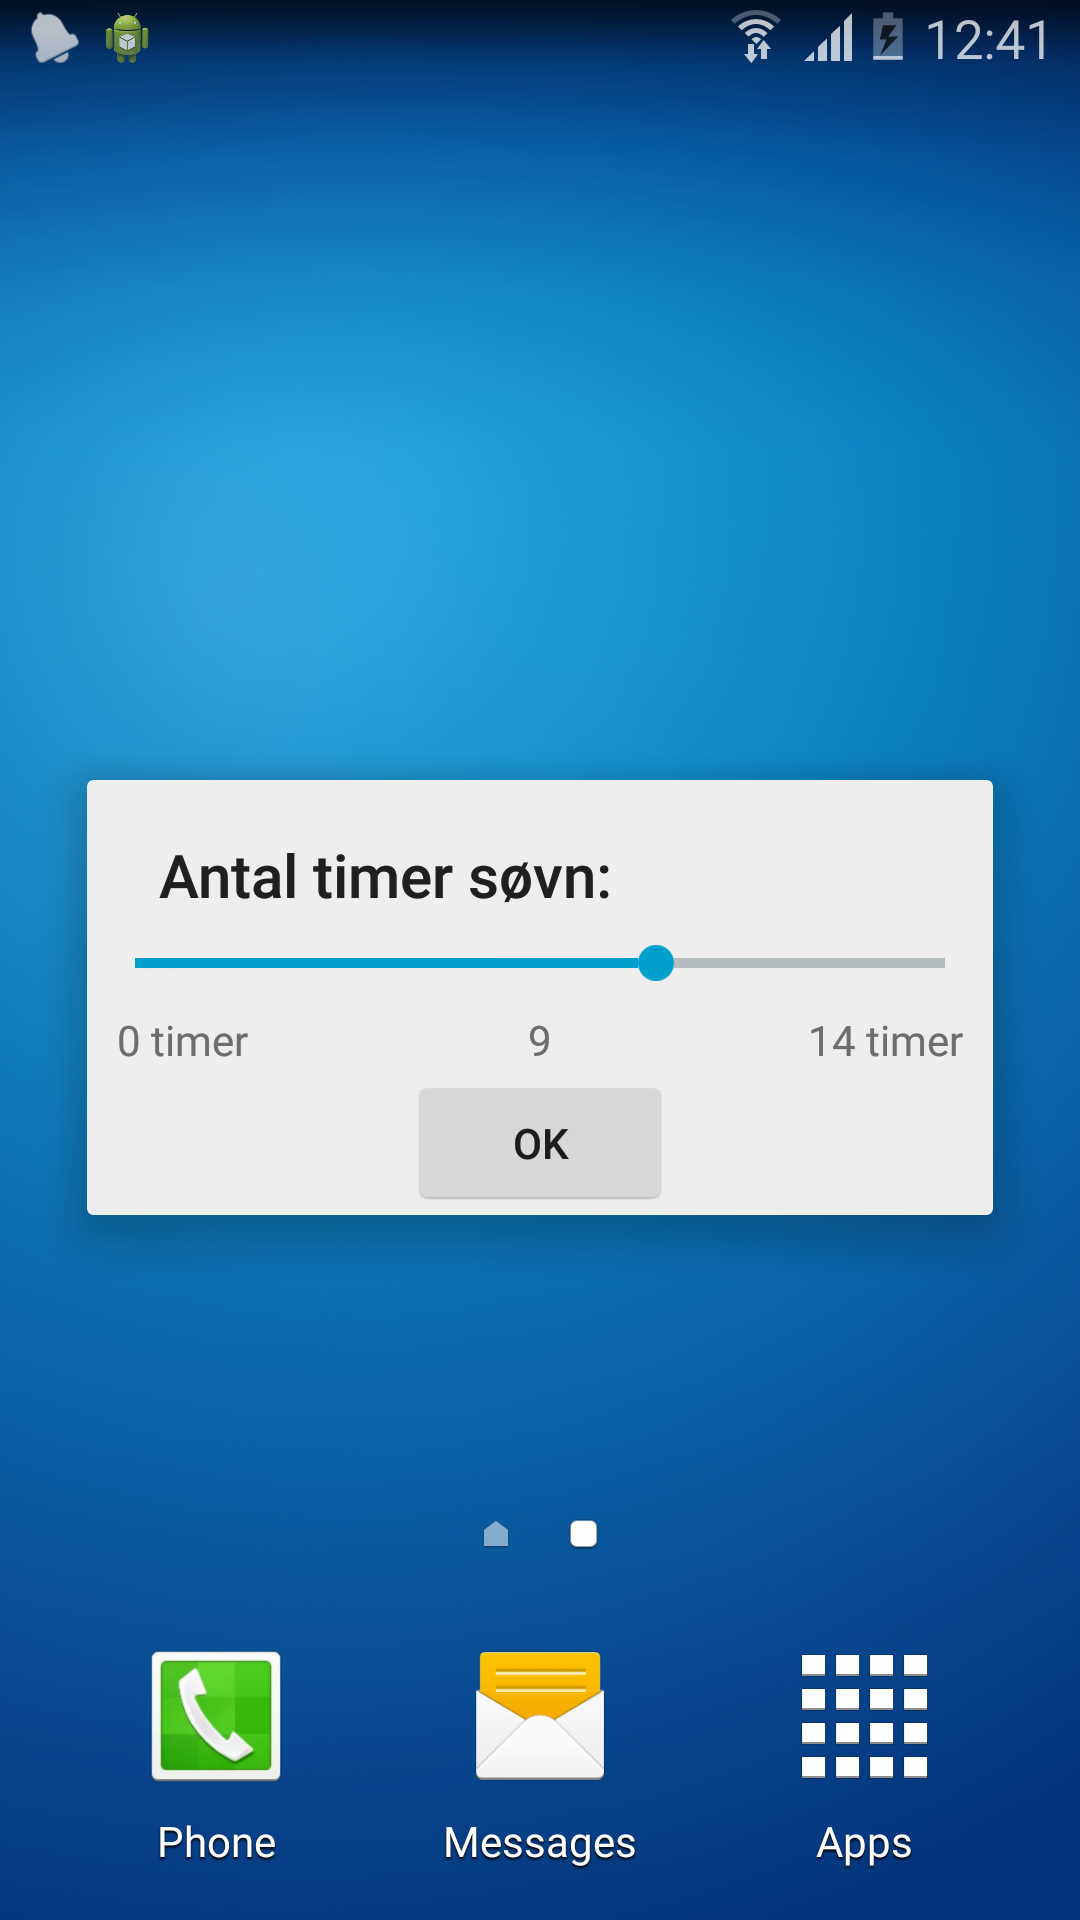
\includegraphics[height=0.8\textheight]{demo_4_popup}
\end{frame}

\begin{frame}{Opsamling}
	
\end{frame}